\newpage
\section{Deuxième génération : architecture non structurée inspirée de Gnutella}

Cette deuxième implémentation ne repose pas encore sur une vraie DHT structurée au sens de \textit{Chord} ou \textit{Pastry}. Elle correspond plutôt à un réseau pair-à-pair non structuré, inspiré de \textit{Gnutella 0.4}, dans lequel chaque n\oe ud participe à la fois au stockage, au routage et aux échanges réseau. Cette approche a constitué une étape utile pour valider les mécanismes de communication, de découverte et de tolérance aux déconnexions avant l'introduction d'un anneau de hachage cohérent.

\subsection{Positionnement général et lien avec Gnutella}

Le système suit un modèle \textit{pure P2P} : il n'existe aucune séparation entre clients et serveurs. Chaque processus est un \textit{servent} (\textit{server} + \textit{client}) capable de recevoir des connexions entrantes et d'initier lui-même des connexions sortantes.

\begin{table}[htbp]
    \centering
    \begin{tabular}{|l|l|l|}
        \hline
        \textbf{Aspect} & \textbf{Implémentation réalisée} & \textbf{Gnutella 0.4} \\
        \hline
        Topologie & Maillage non structuré & Maillage non structuré \\
        \hline
        Routage & Inondation limitée par TTL & Inondation limitée par TTL \\
        \hline
        Découverte & \texttt{PING}/\texttt{PONG} & \texttt{PING}/\texttt{PONG} \\
        \hline
        Recherche & \texttt{GET} & \textit{Query} \\
        \hline
        Réponse & \texttt{REPLY} direct & \textit{QueryHit} \\
        \hline
        Centralisation & Aucune & Aucune \\
        \hline
    \end{tabular}
    \caption{Résumé comparatif entre l'approche naïve développée et les principes de \textit{Gnutella 0.4}.}
    \label{tab:naive_dht_vs_gnutella}
\end{table}

Cette parenté avec \textit{Gnutella} n'est pas seulement conceptuelle. Elle décrit bien l'intuition de départ : construire d'abord un système entièrement décentralisé, simple à expérimenter, puis observer empiriquement ses limites avant de passer à une DHT structurée.


\subsection{Problème initial : l'absence de vue globale}

Le premier problème rencontré ne vient pas du transport réseau, mais du placement des données. Dans une topologie trop clairsemée, chaque pair ne connaît qu'un sous-ensemble des autres n\oe uds. Or si le choix du propriétaire d'une clé dépend de la vue locale du pair qui effectue le calcul, deux machines peuvent aboutir à des décisions différentes pour la même donnée.

\begin{figure}[H]
    \centering
    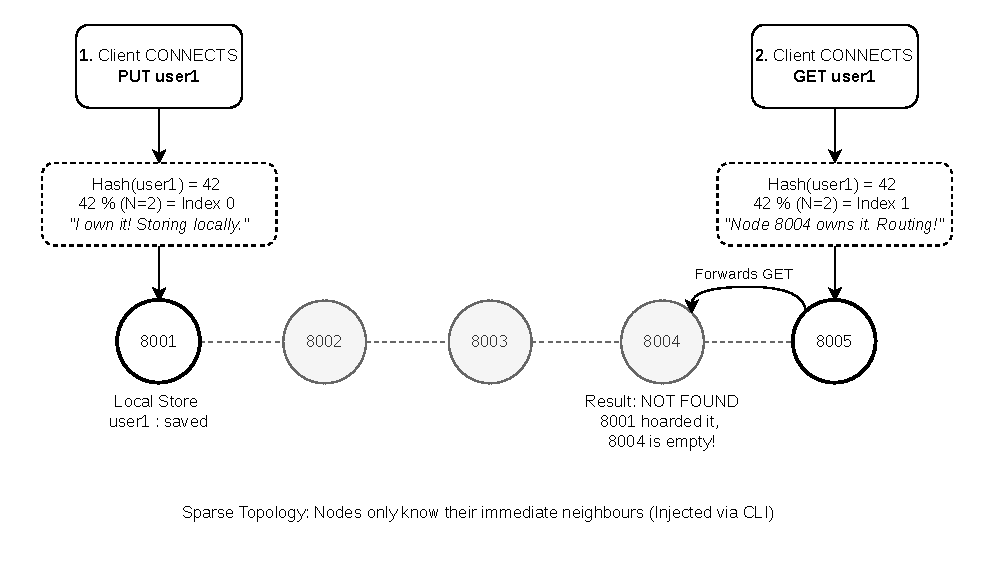
\includegraphics[width=0.92\textwidth]{figures/naive-dht-global-view-problem.drawio.pdf}
    \caption{Problème de vue globale dans une topologie clairsemée. Le n\oe ud \texttt{8001} stocke localement \texttt{user1} après avoir calculé \texttt{Hash(user1) = 42} avec sa propre vision du système. Plus tard, le n\oe ud \texttt{8005} effectue un \texttt{GET} pour la même clé, mais avec une vue réseau différente il conclut que le propriétaire devrait être \texttt{8004} et relaie donc la requête dans une mauvaise direction. L'exemple montre qu'en l'absence d'un espace d'adressage partagé et stable, deux n\oe uds peuvent prendre des décisions incompatibles pour une même clé.}
    \label{fig:naive_dht_global_view}
\end{figure}

Ce constat a motivé un premier choix d'implémentation : tester explicitement une \textbf{structure en mesh} afin d'améliorer la cohérence de la vue réseau. Les schémas présentés dans cette section ne sont donc pas seulement illustratifs ; ils correspondent à des scénarios de test que nous avons utilisés pour vérifier le comportement du système lorsque tous les n\oe uds se connaissent, puis lorsqu'un n\oe ud disparaît.

On peut formaliser cette intuition simplement. Si l'on note \(V\) l'ensemble des n\oe uds actifs et \(E\) l'ensemble des liens de voisinage, alors un mesh complet correspond au graphe non orienté
\[
G = (V,E), \qquad E = \{\{u,v\} \mid u,v \in V,\; u \neq v\}.
\]
Pour \(|V| = N\), le nombre total d'arêtes vaut alors
\[
|E| = \binom{N}{2} = \frac{N(N-1)}{2}.
\]
Chaque n\oe ud a donc un degré exactement égal à
\[
\deg(v) = N-1.
\]
Cette propriété explique pourquoi la vue locale devient beaucoup plus cohérente : en régime stable, chaque pair voit directement tous les autres.

\subsection{Passage à un mesh : ce que cela corrige, et ce que cela casse}

Dans une topologie en maillage complet, chaque n\oe ud possède a priori la même vue des participants actifs. Cette organisation réduit donc fortement le problème de vue globale : tant que le réseau reste stable, les pairs appliquent le même calcul de placement et convergent plus facilement vers le même propriétaire logique. Elle corrige aussi partiellement le problème du modulo naïf, car la cohérence de \texttt{N} est meilleure tant que tous les pairs partagent la même vision du système.

En revanche, cette amélioration reste fragile. Dès qu'un n\oe ud rejoint ou quitte le réseau, la valeur de \texttt{N} change et la fonction de placement \texttt{hash(key) \% N} peut désigner un autre propriétaire. Le maillage complet réduit donc l'incohérence \emph{à l'instant donné}, mais ne supprime pas la dépendance structurelle au nombre de n\oe uds.

Cette fragilité se montre immédiatement par un petit raisonnement. Pour une clé de hachage \(h\), le propriétaire logique dans le schéma naïf est
\[
owner_N(h) = h \bmod N.
\]
Après le départ d'un n\oe ud, le système calcule au contraire
\[
owner_{N-1}(h) = h \bmod (N-1).
\]
Les deux valeurs ne coïncident pas en général. Il suffit d'un contre-exemple pour le voir : avec \(h=10\) et \(N=4\), on obtient
\[
10 \bmod 4 = 2,
\qquad
10 \bmod 3 = 1.
\]
Le propriétaire logique change donc alors même que la donnée n'a pas physiquement bougé. Plus généralement, l'ensemble des clés qui restent stables après le passage de \(N\) à \(N-1\) est
\[
S = \{h \in \mathbf{N} \mid h \bmod N = h \bmod (N-1)\},
\]
et cet ensemble est strictement plus petit que l'ensemble de toutes les clés ; il n'existe donc aucune garantie globale de stabilité sous churn.

\begin{figure}[H]
    \centering
    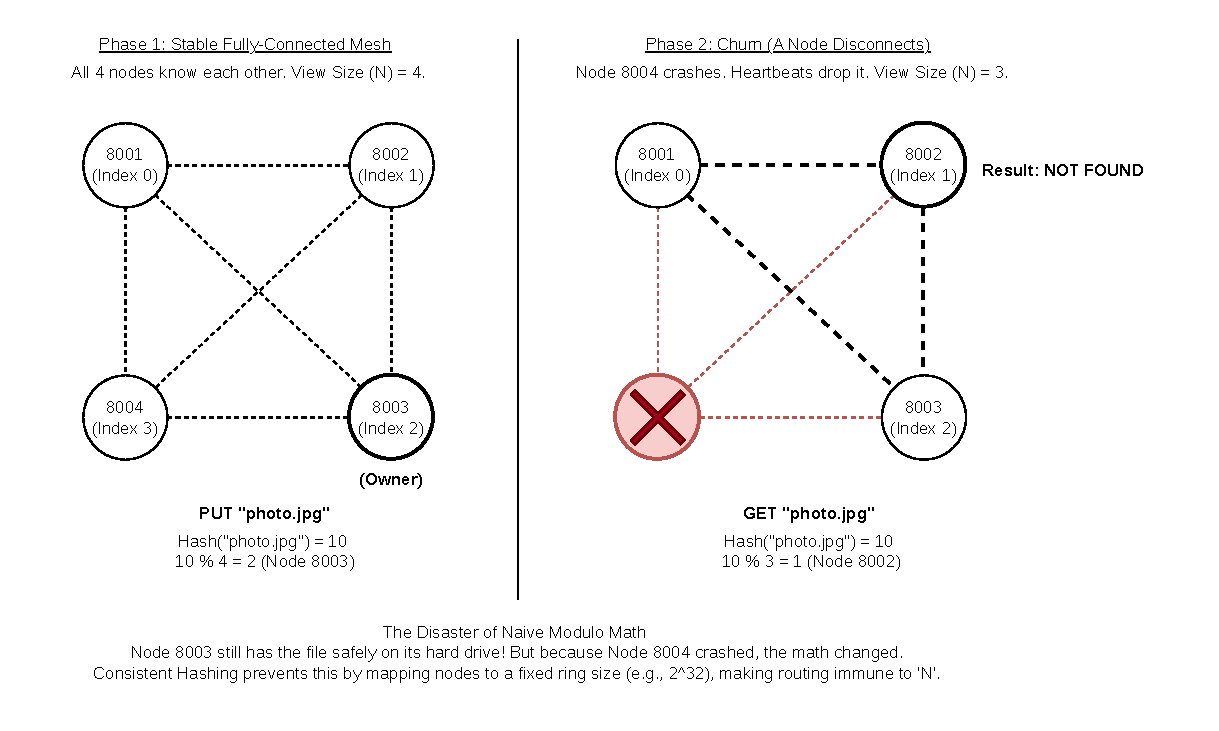
\includegraphics[width=0.95\textwidth]{figures/naive-dht-churn-problem.drawio.pdf}
    \caption{Impact du \textit{churn} sur un placement basé sur \texttt{hash(key) \% N}. À gauche, avec quatre n\oe uds connectés en mesh, la clé \texttt{photo.jpg} est associée au n\oe ud \texttt{8003}, qui la stocke localement. À droite, après la panne du n\oe ud \texttt{8004}, la taille de la vue passe de \texttt{4} à \texttt{3} ; le même calcul désigne alors \texttt{8002} comme propriétaire logique. Le mesh améliore donc la cohérence de la vue tant que le système est stable, mais il ne protège pas contre l'instabilité du placement lorsque \texttt{N} varie.}
    \label{fig:naive_dht_churn}
\end{figure}

Autrement dit, la structure en mesh règle en grande partie le problème de vue globale en régime stable, mais elle fait aussi apparaître plus clairement le vrai défaut du schéma naïf : la dépendance du placement au cardinal du réseau. Les tests de churn ont précisément servi à mettre ce point en évidence.

Du point de vue de la complexité, le mesh complet présente aussi un coût structurel élevé. Comme chaque n\oe ud maintient \(N-1\) voisins, la mémoire consacrée aux tables de voisinage est en \(\Theta(N)\) par pair, soit \(\Theta(N^2)\) à l'échelle du système. De même, un heartbeat envoyé à tous les voisins toutes les \(\Delta = 5\) secondes produit environ
\[
N(N-1)
\]
messages de contrôle par période si l'on compte chaque émission directionnelle. Le coût de maintenance croît donc quadratiquement avec la taille du réseau.

\subsection{Le flooding comme correction partielle}

Une fois ce problème observé, la question n'était plus seulement \og où stocker ? \fg{}, mais aussi \og comment retrouver une donnée quand le calcul local du propriétaire devient faux ou incomplet ? \fg{}. C'est là que l'inondation limitée joue un rôle utile.

Dans cette version, lorsqu'un n\oe ud reçoit une requête \texttt{GET} et qu'il ne possède pas localement la donnée recherchée, il la retransmet à l'ensemble de ses voisins connus. Le mécanisme est donc une \textbf{inondation contrôlée}. Ce n'est pas une solution parfaite au problème de placement, mais c'est une \textbf{solution de rattrapage} : même si un n\oe ud se trompe sur le propriétaire logique, la requête peut encore atteindre le bon détenteur effectif de la donnée à force de propagation dans le mesh.

\begin{itemize}
    \item \textbf{Diffusion.} Une requête est rediffusée de pair en pair jusqu'à trouver un propriétaire potentiel.
    \item \textbf{TTL.} Un plafond \texttt{MAX\_HOPS = 10} limite le nombre de sauts pour éviter les boucles infinies et contenir le trafic.
    \item \textbf{Élimination des doublons.} Le \texttt{PeerRegistry} mémorise les identifiants déjà vus, par exemple sous la forme \texttt{Type|Origin|Seq}, afin d'ignorer immédiatement les messages dupliqués.
\end{itemize}

On peut borner ce coût de recherche. Dans un graphe de degré moyen \(d\), une inondation de profondeur maximale \(T\) génère, dans le pire cas sans élimination efficace des doublons, un nombre de transmissions majoré par une série géométrique :
\[
1 + d + d^2 + \dots + d^T = \sum_{i=0}^{T} d^i.
\]
Si \(d > 1\), cette somme vaut
\[
\sum_{i=0}^{T} d^i = \frac{d^{T+1}-1}{d-1},
\]
soit un coût exponentiel en \(T\). Dans un mesh complet, on peut prendre \(d = N-1\), ce qui donne une borne très pessimiste mais révélatrice : la redondance potentielle devient rapidement prohibitive quand \(N\) grandit.

Grâce au cache de messages déjà vus, l'implémentation réelle est heureusement plus proche d'un parcours borné des arêtes accessibles que d'une explosion purement exponentielle. Dans ce cas, une requête \texttt{GET} touche au plus chaque lien utile un nombre constant de fois, ce qui ramène l'ordre de grandeur à \(O(|E|)\). Pour un mesh complet, cela reste
\[
O(|E|) = O\!\left(\frac{N(N-1)}{2}\right) = O(N^2).
\]
Même avec ce filtrage, le pire cas reste donc quadratique en nombre de n\oe uds. On peut l'écrire plus explicitement dans le cas d'un mesh complet. Comme \(|E| = \frac{N(N-1)}{2}\), une recherche \texttt{GET} qui doit potentiellement explorer tout le réseau avant de conclure à un échec, ou avant d'atteindre le seul n\oe ud possédant la donnée en dernier, effectue dans le pire cas un nombre de transmissions proportionnel à
\[
T_{\text{worst}}(N) \approx 2|E| = N(N-1).
\]
Le facteur \(2\) vient du fait qu'un lien bidirectionnel peut être sollicité dans les deux sens au cours de la propagation et des relais. On obtient donc
\[
T_{\text{worst}}(N) \in \Theta(N^2).
\]
Autrement dit, doubler le nombre de n\oe uds multiplie approximativement par quatre le coût maximal d'une recherche exhaustive, ce qui confirme que cette stratégie ne passe pas bien à l'échelle.

\begin{figure}[htbp]
    \centering
    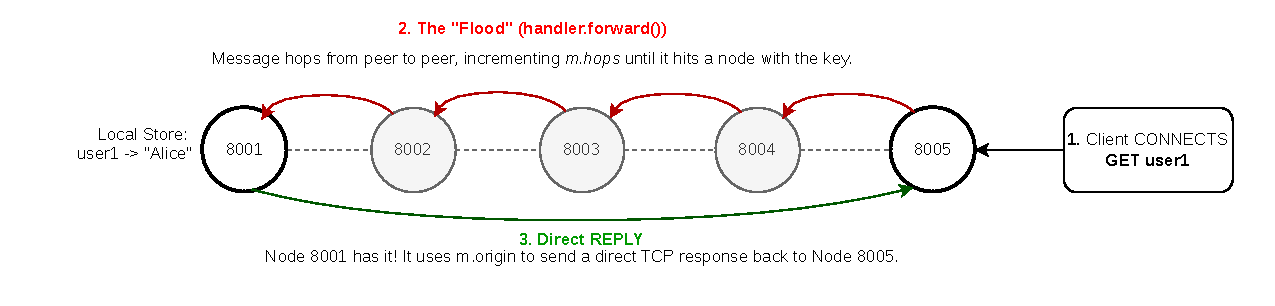
\includegraphics[width=0.92\textwidth]{figures/naive-dht-flooding-search.drawio.pdf}
    \caption{Recherche par inondation dans l'approche naïve. Le n\oe ud \texttt{8005} émet une requête \texttt{GET user1} ; celle-ci est relayée de proche en proche par les pairs intermédiaires, avec incrément du compteur de sauts, jusqu'au n\oe ud \texttt{8001} qui possède la donnée dans son stockage local. Dans ce sens, le flooding corrige partiellement les erreurs de placement ou de vue locale : même si le demandeur ne connaît pas le bon propriétaire, la propagation augmente ses chances d'atteindre le n\oe ud qui détient effectivement la donnée.}
    \label{fig:naive_dht_flooding}
\end{figure}

Ces bornes montrent bien l'ambivalence du flooding dans cette architecture naïve. D'un côté, il constitue un mécanisme de rattrapage robuste : si le réseau reste connexe, qu'aucun lien critique n'échoue pendant la recherche, et que le TTL est au moins égal au diamètre \(D\) du graphe, alors une requête émise depuis un n\oe ud source finit nécessairement par atteindre tout n\oe ud cible détenant la donnée. Dans un mesh complet, le diamètre vaut
\[
D = 1,
\]
ce qui explique pourquoi le flooding y est particulièrement efficace : tant que le système reste stable, la découverte est presque immédiate.

D'un autre côté, cette propriété se paie cher. Le flooding ne résout le problème que partiellement : il compense une mauvaise localisation par davantage de trafic réseau. Le système devient donc plus tolérant aux incohérences, mais au prix d'un coût en messages qui croît vite avec la taille du réseau. Cette tension entre \emph{robustesse de découverte} et \emph{coût quadratique ou pire} résume précisément la limite de l'approche naïve.

\subsection{Réponse directe, protocole et concurrence}

Un point positif de l'implémentation est que la phase de réponse est plus efficace que la phase de recherche. Lorsqu'un n\oe ud trouve la clé demandée, il n'inonde pas le réseau avec la réponse. Il exploite le champ \texttt{origin} du message pour renvoyer directement un \texttt{REPLY} au demandeur au moyen d'une connexion TCP dédiée. On obtient ainsi un schéma classique : découverte diffuse, retour ciblé.

Toutes les communications utilisent TCP afin d'assurer une livraison fiable des messages. Les objets Java sont sérialisés par \texttt{ObjectOutputStream} et désérialisés via \texttt{ObjectInputStream}. Afin de réduire les risques liés à la désérialisation, le \texttt{ConnectionHandler} applique un filtre minimal qui n'accepte que des classes issues d'espaces sûrs, par exemple \texttt{dht.*} et \texttt{java.lang.*}.

Le traitement des connexions suit un modèle \textit{thread-per-connection} :

\begin{itemize}
    \item chaque socket accepté par \texttt{NodeServer} est confié à un \texttt{ConnectionHandler} exécuté dans son propre thread ;
    \item le service \texttt{HeartbeatService} tourne en arrière-plan comme thread démon afin de vérifier périodiquement la vivacité des voisins ;
    \item les structures partagées sont rendues sûres vis-à-vis de la concurrence grâce à une \texttt{ConcurrentHashMap} pour le stockage local et à une \texttt{CopyOnWriteArrayList} pour la liste des pairs.
\end{itemize}

Cette organisation permet de gérer plusieurs pairs simultanément sans bloquer la logique applicative principale, tout en restant relativement simple à implémenter.

\subsection{Découverte et maintien de la vivacité}

Le maintien du réseau repose sur une gestion active de la présence des pairs.

\begin{itemize}
    \item \textbf{Propagation des arrivées et départs.} Lorsqu'un n\oe ud rejoint le système, il annonce sa présence et ses voisins relaient l'information afin d'améliorer progressivement la convergence de la vue réseau.
    \item \textbf{Heartbeat.} Toutes les 5 secondes, \texttt{HeartbeatService} envoie des messages \texttt{PING} aux pairs connus.
    \item \textbf{Détection de panne.} Un pair est retiré du \texttt{PeerRegistry} s'il ne répond plus, ou s'il reste silencieux pendant plus de \texttt{15} secondes (\texttt{PEER\_TIMEOUT\_MS}).
\end{itemize}

Ces mécanismes rendent le réseau dynamique et autonome, mais ils confirment également qu'une topologie non structurée reste sensible au \textit{churn}. La découverte et le mesh améliorent la connectivité ; ils ne suffisent pas à produire un placement stable des clés.

\subsection{Usages réels et intérêt pratique}

Il serait toutefois réducteur de conclure que ce type d'architecture n'a aucun intérêt pratique. Sous sa forme brute, un réseau entièrement de type Gnutella passe mal à l'échelle pour un stockage distribué global, précisément à cause du coût du flooding et de l'instabilité du placement. En revanche, ses idées restent très utiles dans des contextes où la simplicité, la robustesse et la découverte rapide priment sur l'optimalité asymptotique.

On retrouve aujourd'hui ces idées dans des briques très concrètes.

Sur un réseau local, \textbf{mDNS} (\textit{multicast DNS}) est un mécanisme de découverte sans infrastructure (\url{https://datatracker.ietf.org/doc/html/rfc6762}). Son rôle est simple : permettre à des machines présentes sur le même réseau de s'annoncer mutuellement et de découvrir rapidement leurs voisins sans passer par un serveur central. L'idée est très proche de notre approche naïve : on privilégie la simplicité, la visibilité rapide et l'absence de coordination centrale.

Dans l'écosystème \textbf{libp2p}, on retrouve également cette logique pour la découverte locale des pairs (\url{https://libp2p.io/docs/mdns/}). Un n\oe ud peut ainsi détecter d'autres participants proches et établir rapidement ses premières connexions. À un autre niveau, les protocoles \textit{Floodsub} puis surtout \textit{Gossipsub} servent à diffuser des messages dans le réseau pair-à-pair (\url{https://libp2p.io/docs/pubsub/}). Ils reprennent l'intuition du flooding, mais sous une forme mieux contrôlée afin de limiter le trafic inutile.

Dans les \textbf{blockchains modernes}, la couche réseau pair-à-pair conserve elle aussi cette idée de propagation rapide (\url{https://ethereum.org/developers/docs/networking-layer/}). Concrètement, les n\oe uds commencent par découvrir d'autres pairs, puis utilisent un mécanisme de type gossip pour transmettre transactions et blocs à travers le réseau. L'objectif n'est pas de stocker les données via une DHT naïve, mais de propager vite et sans point central une information qui doit atteindre un grand nombre de participants.

Autrement dit, l'approche naïve inspirée de Gnutella reste pertinente comme brique de base pour des tâches bien ciblées : trouver rapidement des voisins, diffuser une information à grande vitesse, ou maintenir une connectivité décentralisée sans coordinateur central. Ce ne sont pas les mêmes objectifs qu'une DHT structurée ; c'est précisément pourquoi, dans les systèmes réels, ces mécanismes coexistent souvent avec des structures plus élaborées au lieu de les remplacer entièrement.

\subsection{Bilan}

Cette première version a permis de valider plusieurs briques essentielles : communication TCP fiable, sérialisation des messages, gestion des connexions concurrentes, découverte des pairs, surveillance de la vivacité et recherche distribuée. Surtout, elle nous a permis de tester deux idées importantes : d'une part, une structure en mesh améliore nettement la cohérence de la vue réseau ; d'autre part, le flooding permet de retrouver une donnée même lorsque le calcul local du propriétaire devient faux.

Du point de vue des performances, cette architecture a toutefois un comportement très contrasté. Dans le meilleur cas, si la donnée est locale ou si le bon pair est immédiatement accessible, une requête \texttt{GET} se résout en pratique en \(O(1)\) sauts. Dans le pire cas, au contraire, la recherche doit explorer une grande partie du réseau ; sur un mesh complet, son coût atteint alors \(\Theta(N^2)\) en nombre de transmissions. De la même manière, la topologie complète offre un diamètre minimal égal à \(1\), ce qui maximise la rapidité de découverte, mais son coût structurel reste quadratique : chaque pair maintient \(N-1\) voisins, soit une mémoire en \(\Theta(N)\) localement et en \(\Theta(N^2)\) à l'échelle du système.

Le rôle de la topologie est donc central. Une topologie clairsemée réduit les coûts de maintenance, mais elle produit des vues locales divergentes et donc des décisions incompatibles sur le placement des clés. À l'inverse, un mesh complet améliore fortement la cohérence de la vue réseau, mais il ne corrige pas le problème fondamental du placement par \texttt{hash(key) \% N} : dès que \(N\) varie, le propriétaire logique d'une clé peut changer. On obtient donc un compromis défavorable entre cohérence locale, coût de maintenance et stabilité globale du placement.

En revanche, pour le placement stable des données et le routage scalable, ces améliorations restent palliatives. Le mesh ne supprime pas la dépendance à \texttt{N}, et le flooding compense l'erreur par un surcoût en messages. Ces limites motivent directement l'introduction de vraies DHT structurées dans la suite du rapport. Des approches comme \textit{Chord} ou \textit{Pastry} remplacent la dépendance à \texttt{N} par un espace d'identifiants fixe et introduisent des mécanismes de routage déterministes, beaucoup mieux adaptés à un environnement distribué dynamique.